%LV begin move to D9
%LV end move content to D9
%LV begin insert of content from D5
\chapter{Day 6: AI Discussion, Smile Detection and Eigenthings}

\section{Schedule}
\bi
\item 0900-0915: Debrief
\item 0915-1000: AI and Society Discussion
\item 1000-1030: Smile Detection---Concepts
\item 1030-1045: Coffee
\item 1045-1115: Machine Learning
\item 1115-1145: Smile Detection---Implementation
\item 1145-1210: Eigenthings
\item 1210-1230: Review/preview
\ei

\section{Debrief and Synthesis [15 mins]}

\bi
\item Please discuss your overnight work with your table-mates, and get help with the ideas that you are still confused by.
\ei

\section{AI and Society Discussion [45 mins]}

\subsection{Framing (5 minutes)}

Today we'll be talking about a constellation of issues that arise when AI technology, like facial recognition, is deployed in society.  As the historian Melvin Kranzberg famously remarked, ``Technology is neither good nor bad; nor is it neutral.''  As you saw in the reading from the night assignment, the effect of AI technology in society intersects a number of sensitive issues around race, class, and gender.  Due to intersection of AI and these sensitive issues, it helps to take a few minutes to consider some guidelines for having fruitful discussions at your tables.

\begin{itemize}
\item Check out \href{https://drive.google.com/file/d/1RZ9VHbWvsJwDbyF6zrmkd5mUdINrzt_f/view}{this poster} put together by some Oliners with suggestions for having conversations on sensitive topics.
\item The readings provide common information and framing, which we find is very helpful to finding common ground when discussing issues that individuals may relate to in very different ways.
\item As you may be relatively new to these ideas, consider adopting a mindset of identifying key questions rather than necessarily coming to conclusions.
\item When talking about the effect of a technology on a group that has been historically oppressed, you should be particularly sensitive in these discussions if you are not a member of this group.  Be conscious of the ways in which your words might be experienced by those who may have faced a history of discrimination due to being a member of this group.
\end{itemize}

\subsection{Unpacking the Readings (15 minutes)}
Write down key concepts and clear up points of confusion on the readings.

\begin{itemize}
\item \href{https://docs.house.gov/meetings/GO/GO00/20190522/109521/HHRG-116-GO00-Wstate-BuolamwiniJ-20190522.pdf}{Joy Buolamwini's written testimony} on bias in facial recognition technology (you may have watched this instead).
\item \href{https://www.fatml.org/resources/principles-for-accountable-algorithms}{Principles for Accountable Algorithms}
\item \href{https://cloud.google.com/inclusive-ml/}{Google's Inclusive ML}
\end{itemize}

\subsection{Share Your Positive Application of AI (10 minutes)}
Go around and share the application of AI that you think has the potential for great positive impact on society. Say a little bit about what you learned and how you think it would have a positive impact (e.g., in what ways and for whom).

\subsection{What Did You Take Away? (15 minutes)}

\textbf{Please have one person take notes on this in some electronic format so they can submit it as part of their day survey}

As a table, discuss what you took away from the readings and your discussion thus far.  Here are some dimensions that you might want to explore.
\begin{enumerate}
\item What parts or quotes from the readings were most surprising / impactful to you?
\item Were you surprised by your reaction to reading any of the material (e.g., felt unexpectedly angry, sad, indifferent)?
\item What are the big questions that have been raised for you (these could be things that were already on your radar or new ones entirely)?  These questions could relate to our society as a whole, your role as a citizen within society, your role as an Olin student, your future career path, etc.).
\item How do these readings intersect with knowledge you've gained from other contexts (e.g., in other courses or in your daily life experience)?
\end{enumerate}

%\vspace{3em}

%\be
%\item For the function defined below, match the following derivatives with the correct expression
%\[
%f(x,y) = 6x^{2}y^{2} + 2x^{2}y + 9y + 12
%\]
%
%\be
%\item $\frac{\partial}{\partial x} f(x,y)$
%\item $\frac{\partial}{\partial y} f(x,y)$
%\item $\frac{\partial^2}{\partial x \partial y} f(x,y)$
%\item $\frac{\partial^2}{\partial y \partial x} f(x,y)$
%\be
%\item $12x^{2}y + 2x^{2} + 9$
%\item $24xy + 4x$
%\item $12x^{2}y^{2} + 2x^{2}y + 9$
%\item $12xy^2 + 4 xy$
%\ee
%\ee
%
%\item Match the following terms with the definiitions below:
%\be
%\item $\sigma_d^2 $
%\item $r_{xy} $
%\item $\mu_d $
%\be
%
%\item $\frac{\sum_{i=1}^n (x_i - \mu_x)(y_i - \mu_y)}{N\sigma_x \sigma_y}$
%\item $\frac{1}{N}\sum_{i=1}^N (d_i - \mu_d)^2$
%\item $\frac{1}{N}\sum_{i=1}^N d_i$
%\ee
%\ee
%\ee

%\section{Debrief [15 mins]}
%In class and in the take home exercise, you worked on partial derivatives, gradients, Hessians and linear regression.
%\be
%
%\item With your table, identify a list of key concepts/take home messages/things you learned in the previous take-home assignment.
%\item Try to resolve your confusions with the folks at your table and by talking to an instructor.
%\item How do you do linear regressions on multidimensional data? We will do a board walkthrough of this to help make sure we've got the generalization figured out.
% \ee


\section{Smile Detection---Concepts [30 mins]}

In this session we are going to use our toolbox of linear algebra skills to ``detect'' whether or not a person is smiling in a photograph.  The approach that we will take is very common in \textbf{machine learning} - we will use a dataset to \textbf{train} our algorithm, and we will use a different dataset to \textbf{test} our algorithm. We will first develop the conceptual framework and then implement the approach in MATLAB.

\subsection{The Big Idea}

Let's assume that we have 100 training photos of faces, each consisting of a 5 by 5 grid of pixels. Let's pack these into a matrix $\A$ with 100 rows and 25 columns, i.e. every row is a different face and every column is a different pixel.

Let's also assume that we have already classified every training face as ``smiling'' or ``not-smiling''. Let's create a column vector $\b$ with 100 rows (corresponding to each face) which has either $1$ (smiling) or $0$ (not-smiling).

Let's now develop a linear system of algebraic equations by trying to express the vector $\b$ as a linear combination of the columns of $\A$, i.e.

\[\A \x = \b \]

Notice that the vector $\x$ is a column vector with 25 rows - one row for each pixel. Since there are more rows than columns we know that an \textbf{exact} solution does not exist, so we will find the \textbf{approximate} solution by orthogonal projection, i.e. we will solve

\[\A^T \A \x = \A^T \b \]

Now that we have the vector $\x$, let's use it to detect whether a test image is smiling. Assuming that the test image is packed into a single row vector $\t$ (with 25 columns) then the product 

\[\t \x \]

will return a scalar. If this scalar is close to ``1'' then we predict the face is smiling. If this scalar is close to ``0'' then we predict the face is not smiling.

\begin{prob}
In this exercise you will be carefully reading and interpreting this big idea. We are including these questions as a scaffold, pointing out interesting features along the way.
\be
\item Read ``The Big Idea'' again! 
\item Interpret what it means to write down the linear system of equations $\A \x = \b$ and give a meaning to the vector $\x$.
\item Interpret the product $\A^T \A$ and the product $\A^T \b$.
\item The vector $\x$ does not satisfy $\A \x = \b$ exactly. What does the expression $\A \x-\b$ tell you?
\item How would you decide whether your ``trained'' algorithm was worth using on a test dataset?
\item Assume you had 40 test images with 25 pixels each and that you pack them into a matrix $\T$ with 40 rows and 25 columns. Write down the matrix-vector product you would use for smile detection on this test dataset.
\item How would you measure the accuracy of your predictions if we also provided you with the data on whether each test image was smiling or not?
\ee
\end{prob}
\begin{sol}
\be
\item Read, read, read ....
\item We are trying to take a linear combination of the data in order to predict whether each image is smiling or not. The vector $\x$ is the magic set of weights we have to use. Its size is the same as the number of pixels, so maybe it should look like a mask that we can place over an image to tell us whether it is smiling.
\item The product $\A^T\A$ is like a pixel to pixel correlation matrix, except we haven't scaled the data matrix $\A$. The product $\A^T \b$ is the sum of the images that are smiling.
\item The expression $\A \x - \b$ tells us the error in predicting whether a training image is smiling or not.
\item We could add up how often the predictor is correct and divide by the number of images to get an estimate of the accuracy. We would decide on a cut-off before we used it on a test dataset.
\item It is simply $\T \x$.
\item As before. Determine how many we got correct and average it.
\ee
\end{sol}

\section{Machine Learning in general [30 mins]}

Machine learning is an interdisciplinary field concerned with the idea that rather than preprogramming machines to solve tasks explicitly, instead we can program them to learn to solve tasks through experience.  In order to connect this idea to what you've done thus far, first we'll introduce a somewhat more formal definition of machine learning.

\begin{quote}
A computer program is said to learn from experience E with respect to some class of tasks T and performance measure P if its performance at tasks in T, as measured by P, improves with experience E.
\flushright{--- Tom Mitchell}
\end{quote}

Let's take the smile detection problem that you just framed in the preceding section of the document.

\vspace{1em}

\begin{tabular}{l | l}
Symbol from Mitchell's Definition & Smile Detection \\
\hline
$E$ & 5 by 5 grids of pixels with corresponding labels as to whether\\ &or not the person in the grid is smiling \\
\hline
$T$ & Given a new 5 by 5 grid of pixels, predicting whether the \\&  person in the image is smiling. \\
\hline
$P$ & Accuracy on predicting whether a person is smiling (e.g., \\&percent  correct)
\end{tabular}

The last part of the definition states that in order to say a program is  ``learning'', it should ``improve with experience E.''  In the case of smile detection, what this means is that given more images with corresponding indication of whether each person is smiling, our program should get better at predicting whether a face is smiling.  Later in this document when you implement smile detection, you'll see that the framing of smile detection as an LSAE problem absolutely meets this definition (and does a surprisingly good job at it too)!

\begin{prob}
In this exercise you and your table-mates will be working to frame various machine learning problems as systems of linear equations.  In doing so, you should answer the following questions.
\bi
\item What is the thing you want to predict (i.e., what is your $\b$ in $\A \x = \b$).
\item What quantities are you using to make your prediction (i.e., what do each of the rows and columns in the matrix $\A$ represent)?
\item While $\x$ would be determined by solving $\A \x = \b$, come up with a guess as to what $\x$ would be (don't worry about coming up with numbers.  Instead, try to identify the sign of each element of $\x$ and  whether its magnitude is large or small relative to the other entries of $\x$).
\item How would you measure how well your system works?  For example, for smile detection we might apply our learned model $\x$ to new data and see how often it correctly predicts the facial expression (smiling vs. not smiling) of the person in each image.
\item What sorts of issues of bias might you have to worry about in this system?
\ei

\be
\item AirBnB has a \href{https://www.airbnb.com/help/article/1168/how-do-i-turn-smart-pricing-on-or-off}{smart pricing} option that lets folks who list their properties on the site have the price for those listings determined automatically. How might you frame the creation of this smart pricing tool as solving a system of linear equations?  We suggest that you follow the steps outlined at the start of this exercise.  You might want to do a quick AirBnB search if you are not familiar with the site.
\item Netflix suggests content to a user that they are likely to enjoy based on their  viewing history as well as the viewing histories of others.  In the past (although we think possibly not anymore), they used to also incorporate ratings data (1 to 5 stars) of particular movies from both the user receiving the recommendation and other users on the site.  How might you frame the creation of this recommendation system in terms of solving a system of linear equations?  We suggest that you follow the steps outlined at the start of this exercise.  You might want to do a quick Netflix search if you are not familiar with the site.
%\item Maybe predicting demand for a BikeShare service (\href{https://archive.ics.uci.edu/ml/datasets/Bike+Sharing+Dataset}{link to dataset} to see what I'm thinking).
%\item Probably something predicting the severity (burned acreage) of a forest fire (\href{https://archive.ics.uci.edu/ml/datasets/Forest+Fires}{link to dataset} to see what I'm thinking).
%\item Something in the space of music genre recommendation based on listening history for other genres (they could add other data as well).
%\item Sentiment analysis of a sentence of text?  Might be a bit of a leap.  We would also need to contextualize it in a particular application.
%\item Job postings to increase applicants (and applicant diversity) https://www.kaggle.com/c/data-science-for-good-city-of-los-angeles
%\item I find this one weird (but we did it in ML) https://www.kaggle.com/c/petfinder-adoption-prediction
%\item Insincere question prediction: https://www.kaggle.com/c/quora-insincere-questions-classification/data
%\item Something about suggesting job listings (this one has a lot of ethical dimensions)
%\item Resume screening (another really difficult ethical scenario).
\ee
\end{prob}

\section{Smile Detection---Implementation [30 mins]}

Please download the file \href{https://canvas.instructure.com/courses/1774456/files?preview=87166282}{\texttt{smiles.mat}} from the canvas site. If you load this file in MATLAB, you will then have access to the following variables in your workspace.

\begin{verbatim}
train_data       - a 3D array containing 19685 24 x 24 pixel
                   images of faces
smile_flag_train - a vector of the same length as the number
                   of images in train_data, with 1s indicating
                   which images are smiling
test_data        - 500 24 x 24 pixel images of faces
smile_flag_test  - a vector of the same length as the number
                   of images in test_data, with 1s indicating
                   which images are smiling
\end{verbatim}

The `train data' and the associated `smile flag train' are the sets of data you should use to develop your mathematical model.  The `test data' and its associated `smile flag test' are the sets of data you should use to test your algorithm when you are finished!


\begin{prob}
For this exercise we recommend that you use \href{https://canvas.instructure.com/courses/1774456/files?preview=87166298}{our walkthrough notebook}.  The notebook has embedded solutions or you can try it with minimal scaffolding using the suggested process below.  Even if you decide not to use the walkthrough notebook, it's worth running the embedded solutions to pickup some techniques for visualizing your smile detector model.  In any case, as you move into actually implementing the smile detector, we recommend you work as pairs at your table.  Working in a pair will allow you to have someone to bounce ideas off of and also make sure you can see the laptop easily.

Only if you decide NOT to use the walkthrough notebook, you should consider following the procedure below to implement the smile detector.
\be
\item Sketch out a set of steps you would take in order to implement smile detection. (Just words here - no code. e.g. we will have to pack all images into a single matrix)
\item Turn this set of steps into MATLAB pseudo-code. Identify important coding elements without implementing, e.g. we will use \textbf{reshape} to pack the given dataset into a matrix.
\item Review the documentation for MATLAB functions that will be used and be clear on how to use them before implementation, e.g. >> help reshape 
\item Methodically implement smile detection in MATLAB, testing as you go.
\ee
\end{prob}

\begin{sol}
You can use the solutions that are embedded in the walkthrough notebook.
\end{sol}

\section{Introduction to Eigenthings [25 mins]}

We are now going to learn the secret of the genie ...

\subsection{Eigenvalues and Eigenvectors: Definition and Notation}

Consider a square $n\times n$ matrix $\A$. A vector $\v$ is said to be an eigenvector of $\A$ with corresponding eigenvalue $\lambda$ if $\v$ is not a vector of all zeros, and
\begin{align}
\A \v = \lambda \v. 
\label{eqn:EvalDef}
\end{align}
If we treat $\A$ as a transformation matrix then  $\v$ is an eigenvector of $\A$ if it is simply scaled when acted on by the matrix $\A$. In other words,  $\mathbf{v}$ does not change direction when acted upon by $\A$. In general, an $n\times n$ matrix has exactly $n$ eigenvalues (although some of these may be repeated and some of these may be complex!). Note that any scalar multiple of an eigenvector of a matrix is also an eigenvector of that matrix - it's only the direction of the eigenvector that matters.

In the next overnight assignment we are going to develop formal techniques for finding the eigenvalues and eigenvectors of matrices. For now, we are going to focus on concepts and developing some intuition.

\begin{prob}
\begin{enumerate}
\item Show that $\mathbf{v} = \twobyone{\frac{1}{\sqrt 2}}{\frac{1}{\sqrt 2}}$ is an eigenvector of the following matrix by computing the product $\A \v$, and find the corresponding eigenvalue
\begin{align}
A = \twobytwo{1}{1}{2}{0}
\end{align}
\item On the same axes, plot the vector representing $\mathbf{v}=\twobyone{\frac{1}{\sqrt 2}}{\frac{1}{\sqrt 2}}$ and $\A\mathbf{v}$. Does the plot confirm that this is an eigenvector?
\item On the same axes, plot the vector representing $\mathbf{u} = \twobyone{\frac{1}{\sqrt 2}}{1}$ and $\A\mathbf{u}$. Is this is an eigenvector of $\A$?
\end{enumerate}
\end{prob}
\begin{sol}
\begin{enumerate}
    \item Compute that
    $$A \mathbf{v} = \begin{bmatrix} \sqrt{2} \\ \sqrt{2} \end{bmatrix} = 2\mathbf{v}$$
    and so the corresponding eigenvalue is $\lambda=2$.
    \item As we can see in the picture below, both $\mathbf{v}$ and $\mathbf{Av}$ point in the same direction, which confirms $\mathbf{v}$ is an eigenvalue of $\mathbf{A}$
    \begin{center}
    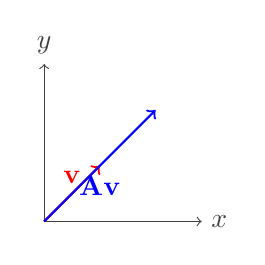
\begin{tikzpicture}[scale=1]
    \draw [->,gray!50!black] (0,0)--(0,2) node[above]{$y$};
    \draw [->,gray!50!black] (0,0)--(2,0) node[right]{$x$};

    \draw [->,red,thick] (0,0)--(0.707,0.707) node[midway,above] {$\mathbf{v}$};
    \draw [->,blue,thick] (0,0)--(1.414,1.414) node[midway,below] {$\mathbf{Av}$};
    \end{tikzpicture}
    \end{center}
    
    \item As we can see in the picture below, $\mathbf{u}$ and $\mathbf{Au}$ point in different directions, so $\mathbf{u}$ is not an eigenvector of $\mathbf{A}$
    \begin{center}
    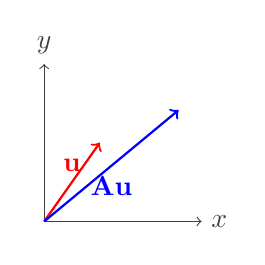
\begin{tikzpicture}[scale=1]
    \draw [->,gray!50!black] (0,0)--(0,2) node[above]{$y$};
    \draw [->,gray!50!black] (0,0)--(2,0) node[right]{$x$};

    \draw [->,red,thick] (0,0)--(0.707,1) node[midway,above] {$\mathbf{u}$};
    \draw [->,blue,thick] (0,0)--(1.707,1.414) node[midway,below] {$\mathbf{Au}$};
    \end{tikzpicture}
    \end{center}
\end{enumerate}
\end{sol}

\subsection{Eigenvalues and eigenvectors of a diagonal matrix}

Recall from our earlier work that the matrix
\[ \A = \twobytwo{2}{0}{0}{3} \]
scales vectors by a factor of 2 in the x-direction and by a factor of 3 in the y-direction. Thus a vector that had a non-zero component only in the $x$ direction will be scaled by a factor of $2$ when transformed by this matrix.  In other words, $\lambda_1 = 2$ is an eigenvalue with corresponding eigenvector $\v_1 = \twobyone{1}{0}$, and that $\lambda_2 = 3$ is an eigenvalue with corresponding eigenvector $\v_2 = \twobyone{0}{1}$. Let's check if the first one is true:

\[ \A \v_1 = \twobytwo{2}{0}{0}{3} \twobyone{1}{0} = \twobyone{2}{0} = 2 \twobyone{1}{0} = 2 \v_1 \]

Therefore $\lambda_1 = 2$ is an eigenvalue with corresponding eigenvector $\v_1 = \twobyone{1}{0}$.

\begin{prob}
Confirm that  $\lambda_2 = 3$ is an eigenvalue with corresponding eigenvector $\v_2 = \twobyone{0}{1}$ by computing the product $\A \v_2$.
\end{prob}
\begin{sol}
We compute that
$$\mathbf{Av}_2 = \twobytwo{2}{0}{0}{3} \twobyone{0}{1} = \twobyone{0}{3} = 3 \twobyone{0}{1} = 3\mathbf{v}_2.$$
\end{sol}

Based on this example, we can heuristically guess that the eigenvalues of an $n\times n$ diagonal matrix are the entries on the diagonal.  The $n$ eigenvectors each have a single 1 in them, with the remaining entries being zero.
\begin{prob}
What are the eigenvalues and eigenvectors of the following diagonal matrices
\begin{enumerate}
\item \[ \A = \threebythree{-3}{0}{0}{0}{-1}{0}{0}{0}{4} \]
\item \[ \A = \threebythree{2}{0}{0}{0}{4}{0}{0}{0}{0} \]
\end{enumerate}
\end{prob}
\begin{sol}
\begin{enumerate}
    \item The eigenvalues are $\lambda_1 = -3$, $\lambda_2 = -1$ and $\lambda_3 =4$ and the corresponding eigenvectors are $\mathbf{v}_1 = \threebyone{1}{0}{0}$, $\mathbf{v}_2 = \threebyone{0}{1}{0}$ and $\mathbf{v}_3 = \threebyone{0}{0}{1}$.
    \item The eigenvalues are $\lambda_1 = 2$, $\lambda_2 = 4$ and $\lambda_3 =0$ and the corresponding eigenvectors are $\mathbf{v}_1 = \threebyone{1}{0}{0}$, $\mathbf{v}_2 = \threebyone{0}{1}{0}$ and $\mathbf{v}_3 = \threebyone{0}{0}{1}$.
\end{enumerate}
\end{sol}

\begin{prob}
\be
\item Assume that $\v = \twobyone{1}{1}$ is an eigenvector with eigenvalue $3$. Construct an appropriate matrix $A$ with this eigenvalue and eigenvector by first rotating $\v$ onto the x-axis, scaling it by $3$, and then rotating back.
\ee
\end{prob}
\begin{sol}
\be
\item First rotate it using a 45 degree clockwise rotation matrix
\begin{align}
\R(-45) = \twobytwo{cosd(-45)}{-sind(-45)}{sind(-45)}{cosd(-45)}
\end{align}
Now that it is along the x-axis we can scale it by 3 using the scaling matrix 
\begin{align}
S = \twobytwo{3}{0}{0}{0}
\end{align}
We then rotate it back using $\R(45)$. Multiplying these matrices together gives
\begin{align}
\A = \twobytwo{1.5}{1.5}{1.5}{1.5}
\end{align}
\ee
\end{sol}

\begin{prob}
What is one eigenvector of the following matrix?
\begin{align}
 \R =   \begin{bmatrix}
\cos \theta & 0 & \sin \theta \\
0 & 1 & 0 \\
-\sin \theta & 0 & \cos \theta \\
\end{bmatrix}
\end{align}
\end{prob}
\begin{sol}
The vector $\mathbf{v} = \begin{bmatrix} 0 \\ 1 \\ 0 \end{bmatrix}$ is an eigenvector of $\mathbf{R}$ because it is the rotation axis and therefore remains unchanged on rotation.
\end{sol}

\section{Review and Preview [20 minutes]}

\pagebreak
\shipoutAnswer
%LV end of insert content from Day5